\documentclass[14pt]{article}
%General Packages
\usepackage{multicol, enumerate, enumitem, hyperref, color, soul, setspace, parskip, fancyhdr}

%Math Packages
\usepackage{amssymb, amsthm, amsmath, bbm, latexsym, units, mathtools}

%All math in Display Style
\everymath{\displaystyle}

% Packages with additional options
%\usepackage[T1]{fontenc}
\usepackage[headsep=0.5cm,headheight=0cm, left=1 in,right= 1 in,top= 1 in,bottom= 1 in]{geometry}
\usepackage[usenames,dvipsnames]{xcolor}

% SageTeX
\usepackage{sagetex}

% Package to use the command below to create lines between items
\usepackage{dashrule}
\newcommand{\litem}[1]{\item#1\hspace*{-1cm}\rule{\textwidth}{0.4pt}}

\pagestyle{fancy}
\lhead{Module\,4\,-\,Quadratic\,Functions}
\chead{}
\rhead{Progress Exam 4}
\lfoot{Testing}
\cfoot{}
\rfoot{Version C}

\begin{document}
\pagestyle{fancy}

\begin{sagesilent}
load("../Code/generalPurposeMethods.sage")
load("../Code/keyGeneration.sage")
keyFileName = "Module4"
version = "C"
\end{sagesilent}

\begin{enumerate}
\setcounter{enumi}{15}


\begin{sagesilent}
moduleNumber=4
problemNumber=16
load("../Code/quadratic/quadraticGraphToEquation.sage")
\end{sagesilent}
% TYPE 1 - Graph to function

\litem{ \sage{displayStem}

	\begin{center} 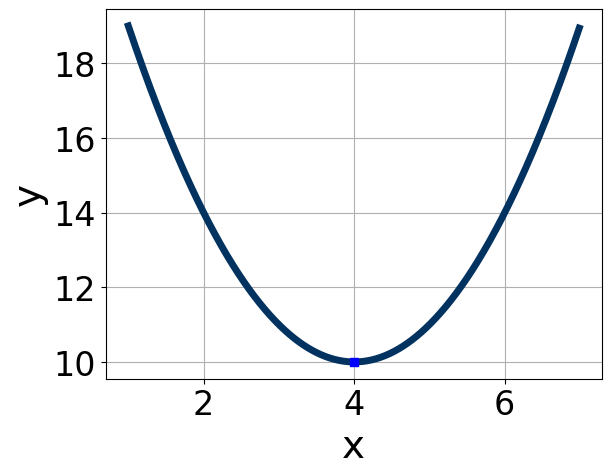
\includegraphics[scale=0.3]{../Figures/quadraticGraphToEquationC.png} \end{center}

	\begin{enumerate}[label=\Alph*.]
		\item \( \sage{choices[0]} \)
		\item \( \sage{choices[1]} \)
		\item \( \sage{choices[2]} \)
		\item \( \sage{choices[3]} \)
		\item \( \sage{choices[4]} \)
	\end{enumerate}

}

\begin{sagesilent}
moduleNumber=4
problemNumber=17
load("../Code/quadratic/quadraticFormula.sage")
\end{sagesilent}

\litem{ \sage{displayStem}
	\[ \sage{displayProblem} \]

	\begin{enumerate}[label=\Alph*.]
    \item \( \sage{choices[0]} \)
    \item \( \sage{choices[1]} \)
    \item \( \sage{choices[2]} \)
    \item \( \sage{choices[3]} \)
    \item \( \sage{choices[4]} \)
	\end{enumerate}
}

\begin{sagesilent}
moduleNumber=4
problemNumber=18
load("../Code/quadratic/quadraticEquationToGraph.sage")
\end{sagesilent}

\litem{ \sage{displayStem}

\[ \sage{displayProblem} \]

\begin{enumerate}[label=\Alph*.]
    \begin{multicols}{2}
	      \item 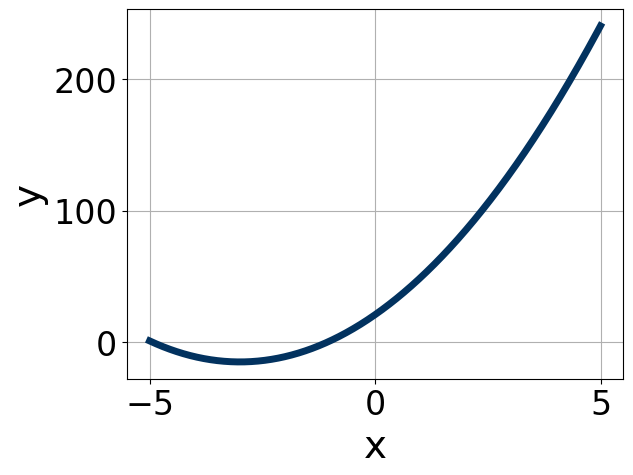
\includegraphics[width = 0.3\textwidth]{../Figures/quadraticEquationToGraphAC.png}
		    \item 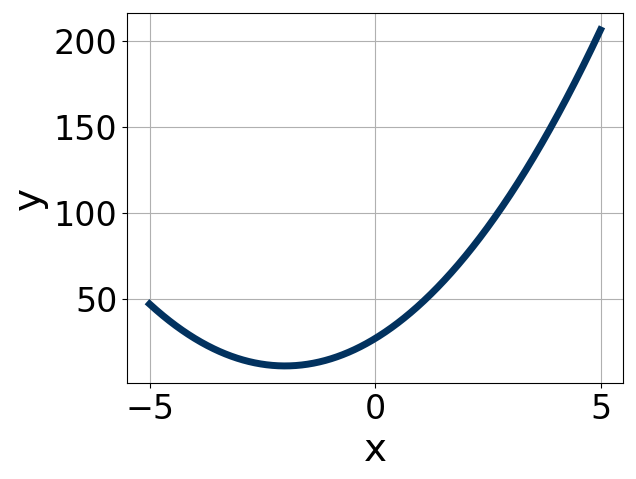
\includegraphics[width = 0.3\textwidth]{../Figures/quadraticEquationToGraphBC.png}
		    \item 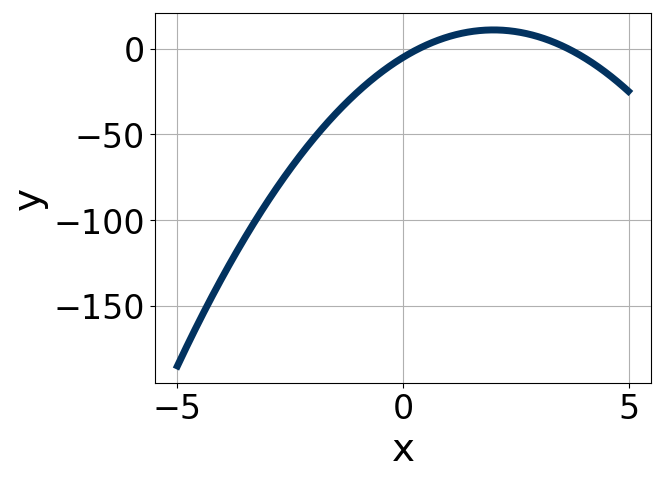
\includegraphics[width = 0.3\textwidth]{../Figures/quadraticEquationToGraphCC.png}
		    \item 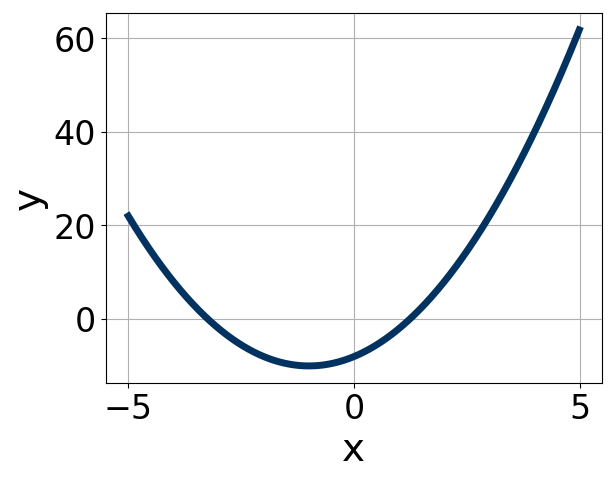
\includegraphics[width = 0.3\textwidth]{../Figures/quadraticEquationToGraphDC.png}
    \end{multicols}
        \item \text{None of the above.}
\end{enumerate}
}

\begin{sagesilent}
moduleNumber=4
problemNumber=19
load("../Code/quadratic/solveQuadraticFactorComposites.sage")
\end{sagesilent}

\litem{ \sage{displayStem}

	\[ \sage{displayProblem} \]

	\begin{enumerate}[label=\Alph*.]
    \item \( \sage{choices[0]} \)
    \item \( \sage{choices[1]} \)
    \item \( \sage{choices[2]} \)
    \item \( \sage{choices[3]} \)
    \item \( \sage{choices[4]} \)
	\end{enumerate}
}

\begin{sagesilent}
moduleNumber=4
problemNumber=20
load("../Code/quadratic/factorLeadingOver1Composite.sage")
\end{sagesilent}

\litem{ \sage{displayStem}

  	\[ \sage{displayProblem} \]

	\begin{enumerate}[label=\Alph*.]
    \item \( \sage{choices[0]} \)
    \item \( \sage{choices[1]} \)
    \item \( \sage{choices[2]} \)
    \item \( \sage{choices[3]} \)
    \item \( \sage{choices[4]} \)
	\end{enumerate}

}

\end{enumerate}

\end{document}

